\section{ARP}
\paragraph{a)}
Resultado do ping:
\begin{figure}[h]
\centering
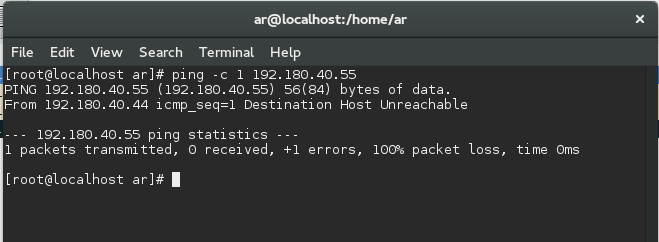
\includegraphics[width=0.7\textwidth]{2_a_screenshot.png}
\label{fig:ping}
\caption{Resultado de \textsf{ping -c 1 192.180.40.55}.}
\end{figure}

\paragraph{b)}
Como podemos verificar no \emph{screenshot} abaixo, capturou-se 3 pacotes ARP de modo a "resolver" o endereço IP 192.180.40.55. Entre as tentativas houve um \emph{timeout} de aproximadamente 1 segundo, uma vez que entre elas (retransmissões) não se conseguiu "resolver" o endereço IP e, depois da terceira tentativa sem resposta, é enviado um pacote ICMP \emph{Host Unreachable} ao IP de origem.\\
É, exatamente, desta forma que funciona o protocolo ARP, ou seja, quando a tradução de um endereço IP não se encontra na cache de ARP é necessário "resolver" esse endereço. Para tal, é enviado uma trama para o endereço MAC de difusão (pacote ARP), todos os nós (terminais e/ou \emph{routers}) recebem e processam a trama, mas apenas o que reconhece o endereço pretendido responde e a informação é adicionada à cache de ARP. Se não ocorrer a resposta no espaço de 1 segundo (\emph{timeout}), a trama é retransmitida e, se à \textbf{terceira} tentativa não receber resposta, "desiste" e é enviado um ICMP \emph{Host Unreachable} (!H) ao IP de origem do pacote.

\begin{figure}[h]
\centering
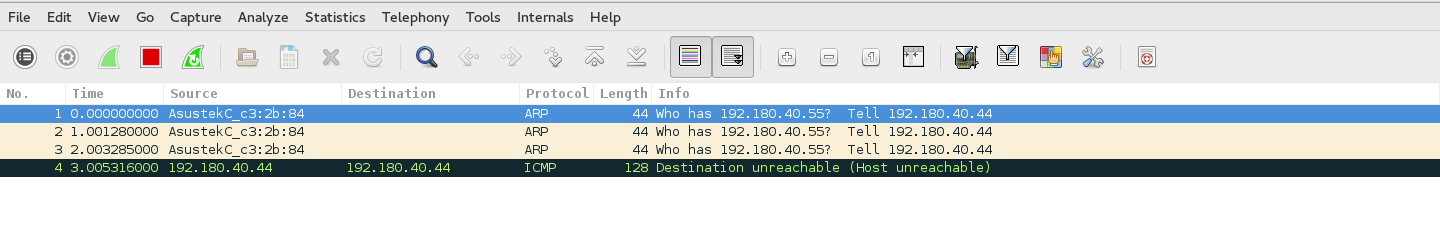
\includegraphics[width=0.8\textwidth, height=0.13\textheight]{2_a__screenshot.png}
\label{fig:wireshark}
\caption{\emph{Screenshot} do \emph{wireshark} a correr na máquina \textsf{Term2}.}
\end{figure}